\documentclass[conference]{IEEEtran}
\IEEEoverridecommandlockouts
% The preceding line is only needed to identify funding in the first footnote. If that is unneeded, please comment it out.
\usepackage{cite}
\usepackage{amsmath,amssymb,amsfonts}
\usepackage{algorithm}
\usepackage{algorithmicx}
\usepackage{algpseudocode}
\usepackage{tikz}
\usetikzlibrary{arrows.meta, positioning}
\usepackage{listings}
\usepackage{graphicx}
\usepackage{textcomp}
\usepackage{xcolor}

\graphicspath{{../images/}}
\def\BibTeX{{\rm B\kern-.05em{\sc i\kern-.025em b}\kern-.08em
    T\kern-.1667em\lower.7ex\hbox{E}\kern-.125emX}}
\begin{document}

\title{Network Flow and Circulation with Demands}


\author{\IEEEauthorblockN{Edwin Sarver}}

\maketitle

%TODO: https://tex.stackexchange.com/questions/13675/use-graphviz-within-tex

\section{Introduction}
The Ford-Fulkerson method and the Edmonds-Karp algorithm that built upon it
by using Breadth-First Search, are valuable algorithms in many fields that 
must know how to maximize the flow through a network.

\section{Algorithms}\label{algo}
Two main algorithms were used in this project: Breadth-First Search (BFS),
and Edmonds-Karp, a derivative work of Ford-Fulkerson.

\subsection{Breadth-First Search}
The breadth-first search algorithm is used to find the path from the given
start node to the given end node that includes the fewest edges. This is 
accomplished by visiting all adjacent nodes to the source, then all the 
adjacent nodes to those nodes and so on until all nodes have been visited.

When performing these steps, it is necessary to note which nodes have been 
visited, the number of jumps to get to that node, and the order in which 
the nodes were visited. A pseudocode version of BFS is shown in 
Algorithm \ref{bfs}. 

\begin{algorithm}
\caption{Breadth-First Search \cite{b1}}\label{bfs}
   \begin{algorithmic}[1]
    \Function{BFS}{$G, s$}
    \For{node in $G.V$} \label{bfs_init_loop}
        \State $node.color = $WHITE
        \State $node.dist = \infty$
        \State $node.prev =$ NIL
    \EndFor
    \State $s.color =$ GRAY
    \State $s.dist =$ 0
    \State $s.prev =$ NIL
    \State $Q = \emptyset$
    \State Enqueue($Q, s$)
    \While{$Q \neq \emptyset$} \label{bfs_while_loop}
    	\State $u =$ Dequeue($Q$)
    	\For{each $v \in u.adjacent\_nodes$} \label{bfs_nested_for}
    		\If{$v.color ==$ WHITE}
    			\State $v.color =$ GRAY
    			\State $v.dist = u.dist + 1$
    			\State $v.prev = u$
    			\State Enqueue($Q, v$)
    		\EndIf
    	\EndFor
		\State $u.color =$ BLACK
    \EndWhile
    \EndFunction
   \end{algorithmic}
\end{algorithm} 

\subsubsection{Theoretical Performance}
The initialization loop (line \ref{bfs_init_loop}) of BFS in Algorithm \ref{bfs} 
will complete in $O(V)$ time because it must run over every vertex in $V$. 
The while loop (line \ref{bfs_while_loop}) will run over each edge in the 
graph and will thus complete in $O(E)$. Therefore the total running time is
$O(V+E)$.


\subsection{Ford-Fulkerson/Edmonds-Karp}
The Ford-Fulkerson method is a set of algorithms used to determine the maximum 
possible flow through a network. There is a derivative method called Edmonds-Karp 
that prescribes that a path-finding algorithm be used to find an augmenting path. 
The method works as shown in Algorithm \ref{ff}.
 

\begin{algorithm}
\caption{Ford-Fulkerson Method \cite{b1}}\label{ff}
	\begin{algorithmic}[1]
		\Function{FordFulkerson}{$G, s, t$}
			\State $f = 0$
			\While{$\exists p \in G_f$}
				\State $f = G_f.augment(p)$
			\EndWhile
			\State \Return $f$
		\EndFunction
	\end{algorithmic}
\end{algorithm}

The first part in Algorithm \ref{ff} is to find an augmenting path. An augmenting 
path is a simple path, one that only visits the constituent nodes and edges once, 
from the source node to the sink node. The flow along an augmenting path can only be 
increased by the minimum capacity along that path, along what is known as the critical
edge. 

After finding the first augmenting path and increasing the flow along that path, a 
residual network is created. The residual graph is created by removing the critical
all critical edges, and adding in edges with residual capacities defined by Equation 
\ref{residual_capacity}.

\begin{equation}
\label{residual_capacity}
c_f = \begin{cases}
		c(u,v) - f(u,v) & if (u,v) \in E,\\
		f(v,u) & if (v,u) \in E,\\
		0 & otherwise.
	\end{cases}
\end{equation}

\subsubsection{Theoretical Performance} % TODO revisit this.
When the flow on an edge in an augmenting path is equal to the capacity of 
that edge, that edge is said to be "critical". A critical edge, after augmenting
occurs, is removed from the residual graph. A given critical edge cannot become
critical again until the shortest path from the source to the sink is 2 greater 
than when that critical edge was found. Any edge in a graph can be critical
at most $V/2$ times and there are $E$ edges. Therefore the time complexity of 
the Edmonds-Karp algorithm is $O(EV)$. The loop in the Ford-Fulkerson can be run
up to $O(E)$ times, and therefore the total time complexity is $O(VE^2)$.

\subsection{Circulation}
The Circulation of supply and demand problem is a logistical problem in 
which a flow network has various nodes that have a given demand value. 
If that demand value is negative, that node has a supply. If the demand
value is positive, that node has a demand.

The problem can be reformulated to be a maximum flow problem. Each negative 
demand value can be thought of as an edge from a source to the node with the
demand value. That edge will have a capacity equal to the absolute value of 
the demand value. Similarly, each positive demand value can be thought of as
an edge from the node with the demand value to a sink node with a capacity 
equal to the demand value. 

If the total of all the supply values is not equal to the demand value, there 
is no circulation in the system. However, if the supply and demand values are 
equivalent, then the maximum flow of the system must be determined. The Edmonds-Karp
algorithm can be used to get the maximum flow. 

If the maximum flow is not equal to the sum of the supply or demand values, there is no
circulation in the system. Only if the maximum flow is equal to the sum of the supply value 
and the sum of the demand values is circulation present in the system. 

\section{Data Structures}
Graphs are represented by structures that show how the graphs are connected. There are 
multiple ways to represent these connections. One way is to use an adjacency matrix.

In an adjacency matrix, the connection between each node to every other node is represented.
In such a structure, there has to be $|V|^2$ slots to hold the connection information. This
method of representation is very convenient for the programmer because determining if a 
connection exists is easy. However, it is only considered space efficient if the graph in
question is very dense. 

The other option is to use an adjacency list. Each node in an adjacency list contains a list 
that holds only the connection information for the nodes to which is is connected. This makes 
adjacency lists well suited for sparse graphs. 

Since flow networks are sparse graphs, adjacency lists are the obvious choice to represent them.

\section{Implementation Difficulties} % TODO revisit this
There were very few obstacles while implementing the algorithms described in section 
\ref{algo}. One issue that was narrowly avoided, however, was ensuring that the circulation
graph implementation was able to correctly inherit from the other graph objects. There
were several methods that had to be \lstinline{virtual}. 

This would have caused an issue in the Ford-Fulkerson implementation if a circulation graph
was passed to it, such as when the circulation algorithm was run. This could have been 
worked around my converting the circulation graph to a flow network, but would have relied
too heavily on convention to ensure errors were not made.


\section{Experimental Performance Analysis}
The theoretical time complexity of Breadth-First Search is $O(V + E)$ and the theoretical
time complexity of the Edmonds-Karp algorithm is $O(VE^2)$. To show that this is the case,
many samples of actual running time must be completed. This will control for the variability
caused by doing the tests on a general-purpose computer. 

\subsection{BFS}
The BFS algorithm was a relatively inexpensive algorithm to run and could, therefore,
be run on a large number of samples. Fig. \ref{bfs_perf} shows the running time of the 
the BFS algorithm versus $V + E$. Since the running time is plotted against the expected
upper bound, it is expected that the asymptotic bound in the graph would be shown as a 
straight line or concave down. Besides a single outlier, likely due to the operating 
system scheduling other tasks, there is a defined, straight line bounding the points of 
this graph. 

\begin{figure}
	\centering
	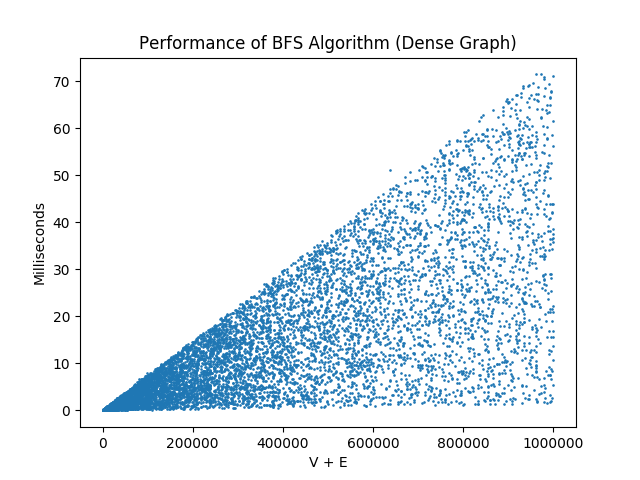
\includegraphics[width=3.25in]{BFS_DenseGraph.png}
	\caption{BFS Performance: Run Time vs $V + E$}
	\label{bfs_perf}
\end{figure}

\subsection{Edmonds-Karp}

The Edmonds-Karp algorithm may have different running characteristics depending on the 
density of the graphs it is to process. Both densities were tried and are shown in Fig. 
\ref{ff_perf_sparse} and \ref{ff_perf_dense}. 

In the sparse graph results (Fig. \ref{ff_perf_sparse}), the running time was, once again,
plotted against the expected time complexity of $O(VE^2)$. In this graph there are distinct,
convex-down asymptotes. This is likely an artifact from the way that the random graphs are 
generated (see section \ref{perf_explanation} for more information). Regardless, the overall convex-down asymptote shows that the points in the plot 
are bounded by $O(VE^2)$.

\begin{figure}
	\centering
	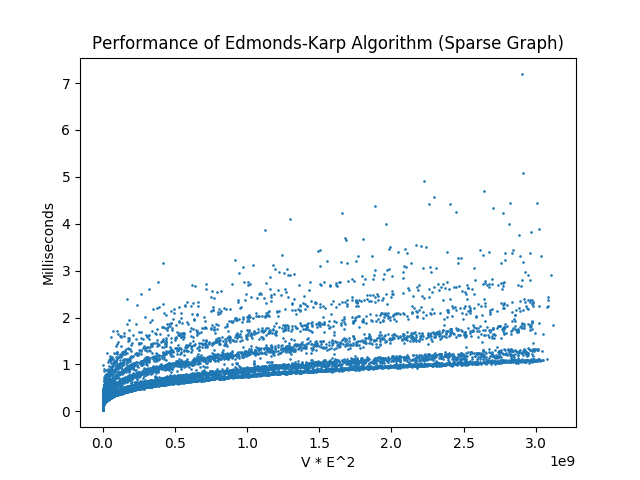
\includegraphics[width=3.25in]{Edmonds-Karp_Sparse.png}
	\caption{Edmonds-Karp Performance on Sparse Graph: Run Time vs $VE^2$}
	\label{ff_perf_sparse}
\end{figure}

The performance tests of the dense graphs took much longer to run, since there are significantly
more edges in these graphs than the sparse graphs. Because of this, much fewer samples could be 
run in a reasonable amount of time. 

As with the sparse graphs, there is a convex-down asymptote when running time is plotted against
$VE^2$. This validates that the overall time complexity of the Edmonds-Karp algorithm is bounded 
by $O(VE^2)$.
\begin{figure}
	\centering
	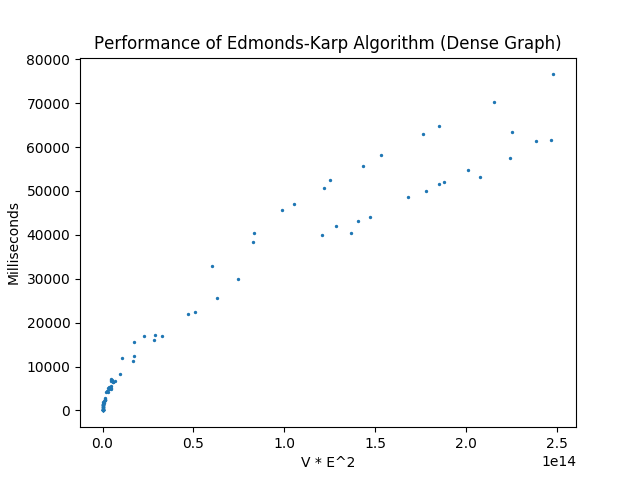
\includegraphics[width=3.25in]{Edmonds-Karp_Dense.png}
	\caption{Edmonds-Karp Performance on Dense Graph: Run Time vs $VE^2$}
	\label{ff_perf_dense}
\end{figure}

The variability of the time required for each step of the Edmonds-Karp algorithm is likely the 
cause of the plots above showing a convex-down asymptote. It is difficult to randomly generate
a worst-case graph. Most graphs will likely run in less than $VE^2$ time, as is shown in the 
results.

\section{Insights}
The Ford-Fulkerson algorithm is a very flexible algorithm. The method by which augmenting paths 
are determined can be replaced for other algorithms, such as in the case of using BFS in Edmonds-Karp.
This allows for improvements to be made to the efficiency of the algorithm without changing the 
basis of how the algorithm works. This is a powerful way to design an algorithm. It allows for 
incremental improvements as more people are able to investigate and experiment with the problem.

Even with this modularity, Ford-Fulkerson and the Edmonds-Karp derivative are still greedy algorithms
that require a long time to run.


\section{Test Cases}
In this project, many forms of testing were utilized: Unit tests, correctness tests,
and performance tests.

\subsection{Unit Tests}
Unit tests were used to ensure that each part of the program functioned as intended even after
changes were made to the code base. Included in these tests were tests to verify the algorithms
described in section \ref{algo}. The graphs that were used in these tests were examples from 
textbook and internet sources with results that were known before the test was written. 

\subsection{Correctness Tests}
The more interesting and valuable test-cases were the randomly generated problems. The goal
of these test-cases were to create graphs of a known size, density, and result without needing
to write them by hand. Because this method of testing could generate more varied graphs, there 
was greater confidence that the algorithms were implemented were correct. The generated graphs 
targeted one of the two major algorithms: BFS or Ford-Fulkerson. Circulation was not targeted
because it was more of an application of the Ford-Fulkerson method.

The graphs targeted at BFS were generated by creating a known path. After this known path was
known, more edges and nodes were added to the graph. When creating the extra nodes and edges, 
the only rule was that the edges could not connect to the nodes on the shortest path. This 
ensured that the shortest path from start to finish was always the known shortest path. 

The graphs targeted at Ford-Fulkerson were generated by using a "bottleneck" edge between 
two sub-graphs. This bottleneck edge has a capacity the is significantly smaller than the 
edges in the two sub-graphs. This ensures that the maximum flow through the full graph
will be limited to the capacity of the bottleneck edge. The maximum flow is, therefore, 
known after generation.

\subsection{Performance Tests}\label{perf_explanation} %TODO revisit this
The performance tests make use of the random graph generation utilities created for the 
correctness tests. For the desired number of samples, a graph is created then a timer is
started, the algorithm in question is then run, then the timer is stopped. The information
concerning the number of vertices and edges, and the running time is then output to a 
JSON file. This file can then be plotted using a python script. 

%\subsection{Design}
% TODO
%\subsection{Results}
% TODO

\section{Conclusion}
The Edmonds-Karp algorithm is a useful algorithm for many applications. The thought process
behind the Edmonds-Karp algorithm is a valuable starting point in understanding other 
flow network algorithms. 

\begin{thebibliography}{00}
    \bibitem{b1} T. H. Cormen, C. E. Leiserson, R. L. Rivest, and C. Stein, Introduction to Algorithms, 3rd ed., The MIT Press, 2009, pp. 594--602, 709--731 
\end{thebibliography}

\end{document}
